\documentclass[aspectratio=169,10pt]{beamer}

\usetheme{Madrid}
\usecolortheme{seahorse}
\usefonttheme{professionalfonts}
\setbeamertemplate{footline}[frame number]
\setbeamertemplate{navigation symbols}{}

%--------------------------------------------------------------
% Packages
%--------------------------------------------------------------
\usepackage{amsmath,amssymb,amsfonts}
\usepackage{mathtools}
\usepackage{bm}
\usepackage{booktabs}
\usepackage{graphicx}
\usepackage{listings}
\usepackage{xcolor}
\usepackage{tikz}
\usepackage{array}
\usepackage{multicol}

\graphicspath{{figures/}}

%--------------------------------------------------------------
% Listings: Python style
%--------------------------------------------------------------
\lstdefinestyle{python}{
  language=Python,
  basicstyle=\ttfamily\scriptsize,
  numbers=left,
  numberstyle=\tiny\color{gray},
  frame=single,
  backgroundcolor=\color{gray!7},
  keywordstyle=\color{blue}\bfseries,
  commentstyle=\color{green!50!black}\itshape,
  stringstyle=\color{red!70!black},
  breaklines=true,
  tabsize=4,
  showstringspaces=false,
  captionpos=b,
}
\lstset{style=python}

%--------------------------------------------------------------
% Convenience macros
%--------------------------------------------------------------
\newcommand{\mHH}{\mathcal H}
\newcommand{\inner}[2]{\langle #1, #2 \rangle}
\newcommand{\norm}[1]{\left\|#1\right\|}
\newcommand{\Fix}{\mathrm{Fix}}
\newcommand{\R}{\mathbb{R}}
\newcommand{\Id}{\mathrm{Id}}
\newcommand{\Sol}{\mathrm{SOL}}

%--------------------------------------------------------------
% Title
%--------------------------------------------------------------
\title[KM Method -- Ch.7]{The Krasnosel'ski\u{i}-Mann Iterative Method}
\subtitle{Chapter 7: Relaxation Parameters of the Krasnosel'ski\u{i}-Mann Iteration}
\author{Based on Dong, Cho, He, Pardalos \& Rassias}
\date{\today}

\begin{document}

%--------------------------------------------------------------
\begin{frame}
  \titlepage
\end{frame}

%--------------------------------------------------------------
\begin{frame}{Table of Contents}
  \tableofcontents
\end{frame}

%==============================================================
\section{Notation Recap and New Concepts}
%==============================================================

\begin{frame}[allowframebreaks]{Notation You'll Need / Recap}

  \textbf{The Krasnosel'ski\u{i}-Mann (KM) iteration (recap).} For a
  nonexpansive operator $T:\mHH\to\mHH$ with $\Fix(T)\neq\emptyset$,
  \[
    x_{n+1} = (1-\lambda_n)x_n + \lambda_n T(x_n), \qquad n\ge 0,
  \]
  where $\lambda_n$ is the \textbf{relaxation parameter}. Three
  regimes: \emph{underrelaxed} if $\lambda_n\le1$, \emph{unrelaxed}
  if $\lambda_n\equiv1$, \emph{overrelaxed} if $\lambda_n\ge1$. This
  chapter is entirely about \emph{how to choose} $\{\lambda_n\}$.

  \vspace{0.3em}
  \textbf{What ``optimal'' means here.} Fix an iterate $x_n$ and a
  fixed point $p\in\Fix(T)$. Among \emph{all} possible choices of
  $\lambda_n\in\R$, exactly one makes the \emph{next} iterate
  $x_{n+1}$ as close as possible to $p$ (in norm). Call that value
  the \textbf{$n$-th optimal relaxation parameter} --- plainly, ``the
  best possible single step, in hindsight, if you already knew where
  you were headed.'' It is a one-step-lookahead notion, not a
  statement about the whole trajectory.

  \begin{alertblock}{The catch}
    Computing the optimal $\lambda_n$ requires knowing a fixed point
    $p$ \emph{before} the iteration has found one --- information you
    do not have in practice. Every formula in this chapter is either
    (a) an idealized optimal parameter that depends on the unknown
    $p$ (useful only for analysis / benchmarking), or (b) a
    computable \emph{approximation} that replaces $p$ by quantities
    you can actually evaluate along the way (e.g.\ $T(x_n)$,
    $T(T(x_n))$), or (c) an adaptive rule driven by an observable
    error measure.
  \end{alertblock}

  \framebreak

  \textbf{The variational inequality (VI) problem --- plain
  language.} Let $C\subseteq\mHH$ be closed and convex, and let
  $F:\mHH\to\mHH$ be a vector field (``operator''). The VI problem
  asks: \emph{find a point $x^*\in C$ such that $F$, evaluated at
  $x^*$, never points ``outward'' relative to any other point of
  $C$} --- i.e.\ moving from $x^*$ towards any other feasible point
  $y\in C$ never decreases along the $F(x^*)$ direction:
  \[
    \inner{F(x^*)}{y-x^*}\ge0 \quad\text{for all } y\in C.
  \]
  \textbf{Why you should care.} VI is a common generalization of two
  things you already know:
  \begin{itemize}
    \item \textbf{Fixed-point problems}: taking $F=\Id-T$ turns the
          VI exactly into $x^*=T(x^*)$ (shown later this chapter).
    \item \textbf{Constrained optimization}: minimizing a
          differentiable $f$ over $C$ has first-order optimality
          condition $\inner{\nabla f(x^*)}{y-x^*}\ge0$ for all
          $y\in C$ --- precisely the VI with $F=\nabla f$.
  \end{itemize}

  \textbf{The residual --- plain language.} A \textbf{residual} is
  any quantity that is zero exactly at a solution and measures
  ``how far'' a candidate point is from solving the problem, so it
  can serve as a stopping test or a progress diagnostic. For the
  fixed-point problem the natural residual is
  $\norm{x_n-T(x_n)}$: it vanishes iff $x_n\in\Fix(T)$. For the
  equivalent equation $F(x)=0$ with $F=\Id-T$, the same quantity is
  $\norm{F(x_n)}$.

\end{frame}

%==============================================================
\section{7.0 Why Relaxation Parameters Matter: A Short History}
%==============================================================

\begin{frame}{Three Regimes, One Crucial Choice}

  \textbf{Intuition.} The relaxation parameter $\lambda_n$ decides
  \emph{how big a step} you take from $x_n$ towards $T(x_n)$.
  Small $\lambda_n$: cautious, safe, slow. Large $\lambda_n$
  (overrelaxation, $\lambda_n>1$): aggressive, can converge much
  faster --- \emph{if} chosen well --- but risks divergence if
  chosen badly.

  \begin{block}{Definition (Under/Un/Overrelaxation)}
    The KM iteration is \emph{underrelaxed} if $\lambda_n\le1$,
    \emph{unrelaxed} if $\lambda_n\equiv1$, \emph{overrelaxed} if
    $\lambda_n\ge1$, for all $n\ge0$.
  \end{block}

  \textbf{Why this chapter exists.} The convergence \emph{rate} of
  the KM iteration depends heavily on $\{\lambda_n\}$, yet results
  on how to select it are limited. The remainder of the chapter
  surveys: (7.0) known optimal/near-optimal choices from the
  literature, (7.1) an approximate optimal sequence for general
  nonexpansive $T$, (7.2) relaxations inherited from variational
  inequality projection methods, and (7.3) a residual-driven line
  search algorithm.

\end{frame}

\begin{frame}{Combettes' Optimal Relaxation Parameter}

  \textbf{Setting.} Let $D$ be a closed subspace and $S$ a closed
  convex subset of $\mHH$, and take $T=P_DP_S$ (compose two metric
  projections) in the KM iteration. Combettes asked: for a fixed
  point $p\in\Fix(P_DP_S)$, which $\lambda_n$ minimizes
  $\norm{x_{n+1}-p}$?

  \begin{block}{Optimal Relaxation Parameter (7.1)}
    \[
      \lambda_n^* = \frac{\inner{x_n - P_DP_S(x_n)}{\,x_n-p}}
                          {\norm{x_n-P_DP_S(x_n)}^2}.
    \]
    \begin{itemize}
      \item $x_n-P_DP_S(x_n)$ is (minus) the step $T$ would take;
      \item $p$ is a fixed point --- \emph{unknown} in practice, so
            $\lambda_n^*$ cannot literally be computed; it is a
            theoretical benchmark.
    \end{itemize}
  \end{block}

  \begin{alertblock}{Lemma 7.1}
    The optimal relaxations $\lambda_n^*$ in (7.1) are always
    \emph{overrelaxation}: $\lambda_n^*\ge1$ for every $n\ge0$.
    Combettes further claimed $\lambda_n^*$ could in theory be very
    large, definitely greater than $2$.
  \end{alertblock}

  Note: optimality \emph{per step} does not automatically guarantee
  the \emph{whole sequence} converges faster --- but for the
  parallel projection method, overrelaxation was numerically found
  to accelerate convergence to a solution.

\end{frame}

\begin{frame}{Approximating $\lambda_n^*$: Armijo and Line-Search Ideas}

  \textbf{Why approximate?} $\lambda_n^*$ in (7.1) needs the unknown
  $p$. Combettes instead used an \textbf{Armijo relaxation skill}:
  shrink $\lambda_n$ until a sufficient-decrease test on
  $\Phi(x)=\tfrac12\norm{x-P_DP_S(x)}^2$ holds.

  \begin{block}{Armijo-Type Test (7.2)}
    \[
      \Phi(x_n)-\Phi(x_{n+1}) \ge \mu\lambda_n\norm{\nabla\Phi(x_n)}^2,
    \]
    where $\mu\in(0,1)$ is a fixed constant. Caveat: this needs
    $\Phi$ \emph{differentiable}, which fails for
    $\Phi(x)=\tfrac12\norm{x-T(x)}^2$ when $T$ is only a general
    nonexpansive (or firmly nonexpansive) map.
  \end{block}

  \textbf{Xu's line-search viewpoint.} Rewrite KM as a descent
  method: $x_{n+1}=x_n-\lambda_n v_n$ with search direction
  $v_n=x_n-T(x_n)$. Choose $\lambda_n$ by solving small 1-D
  optimization problems:
  \begin{block}{Xu's Line-Search Choices (7.3)--(7.4)}
    \[
      \lambda_n = \operatorname*{argmin}_{0\le\lambda\le c}
        \bigl\{\norm{x_n(\lambda)-T(x_n)(\lambda)}^2
               -\beta\lambda^2\norm{x_n-T(x_n)}\bigr\},
    \]
    \[
      \lambda_n = \operatorname*{argmin}_{0\le\lambda\le1}
        \bigl\{\norm{x_n(\lambda)-T(x_n)(\lambda)}^2
               -\beta\lambda(1-\lambda)\norm{x_n-T(x_n)}\bigr\},
    \]
    where $x_n(\lambda):=x_n-\lambda(x_n-T(x_n))$, $c\in(0,1)$,
    $\beta>0$. In practice these 1-D problems are hard to solve
    exactly for general $T$, and numerical solvers (e.g.\ golden
    section search) can be too slow.
  \end{block}

\end{frame}

\begin{frame}{The Online Relaxation KM Iteration}

  \textbf{Idea.} Iutzeler and Hendrickx designed a relaxation
  \emph{update rule} that automatically tunes $\lambda_n$ using only
  quantities observable during the run --- no line search, no
  knowledge of a fixed point. Let $T:\R^N\to\R^N$ be $\sigma$-averaged.

  \begin{block}{Algorithm 3: Online Relaxation KM Iteration}
    Initialize $\varepsilon\in(0,2\min(\sigma,1-\sigma))$, $x_0$,
    $x_1=T(x_0)$, $\lambda_0=\lambda_1=1$. For $n\ge1$:
    \[
      \lambda_{n+1} =
        \frac{(2-\varepsilon)\lambda_n}
             {2\sigma\lambda_n+1-\dfrac{\lambda_{n-1}\norm{x_n-x_{n-1}}}
                                        {\lambda_n\norm{x_{n-1}-x_{n-2}}}}
        + \frac{\varepsilon}{4\sigma},
      \qquad
      x_{n+1} = (1-\lambda_{n+1})x_n+\lambda_{n+1}T(x_n).
    \]
  \end{block}

  \begin{alertblock}{Theorem 7.1 (Iutzeler--Hendrickx)}
    If $T:\R^N\to\R^N$ is $\sigma$-averaged with $\Fix(T)\neq\emptyset$
    for some $\sigma\in(0,1)$, then $\{x_n\}$ from Algorithm 3
    converges to a point in $\Fix(T)$.
  \end{alertblock}

\end{frame}

\begin{frame}{Giselsson et al.'s Line-Search Method and the SuperMann Iteration}

  \begin{block}{Two-Step KM With Line-Search Relaxation (7.6)--(7.7)}
    With $0<\bar\lambda\le\lambda_{\max}$ fixed:
    \[
      \begin{cases}
        y_n=(1-\bar\lambda)x_n+\bar\lambda T(x_n),\\
        x_{n+1}=(1-\lambda_n)y_n+\lambda_n T(y_n),
      \end{cases}
      \quad
      \lambda_n\in[\bar\lambda,\lambda_{\max}] \text{ s.t. }
      \norm{x_{n+1}-T(x_{n+1})}\le(1-\epsilon)\norm{y_n-T(y_n)}.
    \]
    This is a two-step KM iteration: the first-step relaxation is
    fixed, the second is chosen by a line search testing the
    fixed-point residual $\norm{y_n-T(y_n)}$.
  \end{block}

  \begin{alertblock}{Theorem 7.2}
    If $T$ is nonexpansive with $\Fix(T)\neq\emptyset$ and
    $\bar\lambda\in(0,1)$, then $\norm{x_n-T(x_n)}\to0$ and
    $\norm{x_{n+1}-x_n}\to0$.
  \end{alertblock}

  \textbf{A cost caveat.} Evaluating the residual test costs a full
  extra evaluation of $T$ --- so testing many candidate
  $\lambda_n$'s per iteration may be too expensive unless $T=T_2T_1$
  with $T_1$ affine and $T_2$ cheap.

  \textbf{SuperMann (Themelis--Patrinos), sketch.} Generalizes KM
  using $R=\Id-T$ and an update direction $d_n$, with three regimes
  per step: a \emph{blind} update (trust $d_n$ outright when the
  residual has shrunk enough), an \emph{educated} update (accept
  $d_n$ after verifying a residual-decrease safeguard), or a
  relaxed-KM \emph{safeguard} update otherwise. Superlinear
  convergence is possible but the conditions are quite restrictive,
  limiting practical use.

\end{frame}

%==============================================================
\section{7.1 The Approximate Optimal Relaxation Sequence}
%==============================================================

\begin{frame}{7.1 Intuition: The Best Step You Could Take (In Hindsight)}

  \textbf{Setup.} Suppose $x_n$ has already been computed, and take
  \emph{any} fixed point $p\in\Fix(T)$ arbitrarily. He, Cho, et al.\
  ask the same question Combettes asked for $T=P_DP_S$, but now for
  a \emph{general} nonexpansive $T$: which $\lambda_n$ makes
  $\norm{x_{n+1}-p}$ as small as possible?

  \vspace{0.3em}
  \textbf{Why this is a clean question.} For fixed $x_n$, $T(x_n)$,
  and $p$, the quantity $\norm{x_{n+1}-p}^2$ is an explicit
  \emph{quadratic function of the scalar $\lambda_n$} --- so ``best
  single step'' reduces to minimizing a parabola, something we can
  do exactly with calculus. That is the entire content of the
  derivation on the next slide.

  \vspace{0.3em}
  \textbf{Where this is going.} The resulting formula still involves
  the unknown $p$. The rest of Section 7.1: (i) derive the ideal
  formula, (ii) study its structural properties, (iii) replace the
  unknown $p$ by \emph{computable} surrogates to get a genuine,
  implementable algorithm, and (iv) prove that algorithm still
  converges.

\end{frame}

\begin{frame}{7.1 Derivation: The $n$-th Optimal Relaxation Parameter}

  \textbf{Step 1 --- expand the update.} Write
  $x_{n+1}-p=(1-\lambda_n)(x_n-p)+\lambda_n(T(x_n)-p)$ and expand
  the squared norm using the standard two-term identity
  $\norm{(1-t)a+tb}^2=(1-t)\norm{a}^2+t\norm{b}^2-t(1-t)\norm{a-b}^2$:
  \begin{block}{Expansion (7.8)}
    \begin{align*}
      \norm{x_{n+1}-p}^2
      &= (1-\lambda_n)\norm{x_n-p}^2+\lambda_n\norm{T(x_n)-p}^2
         -\lambda_n(1-\lambda_n)\norm{x_n-T(x_n)}^2\\
      &= \lambda_n^2\norm{x_n-T(x_n)}^2
         -\lambda_n\bigl(\norm{x_n-p}^2-\norm{T(x_n)-p}^2+\norm{x_n-T(x_n)}^2\bigr)\\
      &\qquad+\norm{x_n-p}^2.
    \end{align*}
  \end{block}

  \textbf{Step 2 --- read off the quadratic in $\lambda_n$.} This is
  $A\lambda_n^2 - B\lambda_n + \norm{x_n-p}^2$ with
  $A=\norm{x_n-T(x_n)}^2\ge0$ and $B=\norm{x_n-p}^2-\norm{T(x_n)-p}^2+\norm{x_n-T(x_n)}^2$.
  Since $A\ge0$, the minimizer (when $A>0$) is $\lambda_n=B/(2A)$.

  \framebreak

  \textbf{Step 3 --- simplify $B/(2A)$.} Substituting $B$ and $A$
  and splitting the fraction gives the closed form:
  \begin{block}{The $n$-th Optimal Relaxation Parameter (7.9)}
    \[
      \widehat\lambda_{p,n} = \frac{1}{2}
        + \frac{\norm{x_n-p}^2-\norm{T(x_n)-p}^2}{2\norm{x_n-T(x_n)}^2}.
    \]
    \begin{itemize}
      \item The $\tfrac12$ is the ``baseline'' half-step;
      \item the fraction adjusts up or down depending on whether
            $p$ is closer to $x_n$ or to $T(x_n)$;
      \item this is called the $n$-th optimal relaxation parameter
            \emph{corresponding to $p$}, since it explicitly involves
            $p$.
    \end{itemize}
  \end{block}

  \textbf{Sanity check.} For $T=P_DP_S$ this formula reduces to
  exactly Combettes' $\lambda_n^*$ in (7.1) --- the general
  derivation recovers the earlier special case.

\end{frame}

\begin{frame}{7.1 Definitions 7.1 \& 7.2: Removing the Dependence on $p$}

  \textbf{Idea.} $\widehat\lambda_{p,n}$ still depends on which fixed
  point $p$ we picked. To get a single well-defined sequence, take
  an infimum over all $p\in\Fix(T)$.

  \begin{block}{Definition 7.1 (Closed Affine $C$)}
    Let $C$ be a closed affine set and $T:C\to C$ nonexpansive. The
    \textbf{$n$-th optimal relaxation parameter} of the KM iteration
    is
    \[
      \widehat\lambda_n = \inf_{p\in\Fix(T)}\widehat\lambda_{p,n}.
    \]
  \end{block}

  \begin{block}{Definition 7.2 (General Closed Convex $C$)}
    For general closed convex $C$, $\widehat\lambda_{p,n}$ can
    overshoot $[0,1]$ (or $[0,1/\sigma]$), which would push $x_{n+1}$
    outside $C$. So cap it:
    \[
      \widehat\lambda_n =
      \begin{cases}
        \min\{\inf_{p\in\Fix(T)}\widehat\lambda_{p,n},\,1\}, & T\text{ nonexpansive},\\
        \min\{\inf_{p\in\Fix(T)}\widehat\lambda_{p,n},\,1/\sigma\}, & T\ \sigma\text{-averaged}.
      \end{cases}
    \]
  \end{block}

  These sequences $\{\widehat\lambda_n\}$ still cannot be computed
  in practice (they involve $\Fix(T)$), but they let us prove
  structural facts about how large/small the ``true'' optimum can be.

\end{frame}

\begin{frame}{7.1 Lemma 7.2: What Do We Know About $\{\widehat\lambda_n\}$?}

  \begin{alertblock}{Lemma 7.2}
    Let $C$ be closed convex, $T:C\to C$, and $\{\widehat\lambda_n\}$
    as in Definition 7.1 or 7.2. Then:
    \begin{enumerate}
      \item If $T$ is nonexpansive, $\widehat\lambda_n\ge\tfrac12$.
      \item If $T$ is $\sigma$-averaged, $\widehat\lambda_n\ge
            \tfrac{1}{2\sigma}$ for each $n\ge0$.
      \item If $T$ is \emph{quasi-isometric}
            ($\norm{T(x)-p}=\norm{x-p}$ for all $x\in C,\,p\in\Fix(T)$),
            then $\widehat\lambda_n=\tfrac12$ for every $n$.
      \item If $\Id-T$ is injective on $C$ and
            $(\Id-T)^{-1}:\operatorname{ran}(\Id-T)\to C$ is
            $L$-Lipschitz, then $\widehat\lambda_n\le L$ for every $n$.
    \end{enumerate}
  \end{alertblock}

  \textbf{Reading the bounds.} Part (2) shows the lower bound
  \emph{grows} as the averaging constant $\sigma$ shrinks --- so to
  get the largest guaranteed lower bound on the true optimal
  parameter, one wants the \emph{smallest valid} $\sigma$ for which
  $T$ is $\sigma$-averaged.

\end{frame}

\begin{frame}{7.1 From Ideal to Practical: The Approximation Formula}

  \textbf{The trick.} We cannot use $p$ in (7.9) because it is
  unknown. But $T(x_n)$ and $T(T(x_n))$ \emph{are} computable, and
  --- if $x_n$ were already close to $\Fix(T)$ --- $T(x_n)$ would be
  a reasonable stand-in for $p$, and $T(T(x_n))$ a stand-in for
  $T(p)=p$. So substitute $p\to T(x_n)$ and $T(x_n)\to T(T(x_n))=T^2(x_n)$
  directly into (7.9):

  \begin{block}{The Approximate Optimal Relaxation Parameter (7.12)}
    \[
      \lambda_n = \frac{1}{2} +
        \frac{\norm{x_n-T(x_n)}^2 - \norm{T(x_n)-T^2(x_n)}^2}
             {2\norm{(x_n-T(x_n))-(T(x_n)-T^2(x_n))}^2}, \qquad n\ge0.
    \]
    \begin{itemize}
      \item $x_n-T(x_n)$: the fixed-point residual at $x_n$;
      \item $T(x_n)-T^2(x_n)$: the fixed-point residual ``one step
            ahead,'' at $T(x_n)$;
      \item the denominator is the norm of the \emph{difference of
            residuals} --- how much the residual changed between
            $x_n$ and $T(x_n)$.
      \item Only three operator evaluations are needed
            ($T(x_n)$, then $T$ of that): fully computable, no
            oracle for $\Fix(T)$ required.
    \end{itemize}
  \end{block}

  Numerical experiments in the source paper show (7.12) clearly
  outperforms both a fixed relaxation parameter and the online
  relaxation formula (7.5).

\end{frame}

\begin{frame}{7.1 Running Example: Setting Up}

  \textbf{Running example (unit-disk projection), recap.} Let
  $\mHH=\R^2$, $C=\{x:\norm{x}\le1\}$, $T=P_C$:
  \[
    T(x)=P_C(x)=
    \begin{cases}
      x, & \norm{x}\le1,\\
      x/\norm{x}, & \norm{x}>1.
    \end{cases}
  \]
  Take $x_0=(3,4)$, so $\norm{x_0}=5$; the fixed point reached along
  this ray is $x^*=x_0/\norm{x_0}=(0.6,0.8)$.

  \begin{alertblock}{A convenient structural fact}
    Whenever $\norm{x_n}>1$, we have $T(x_n)=x_n/\norm{x_n}\in C$,
    hence $T(x_n)\in\Fix(T)$ automatically (any point already inside
    $C$ is a fixed point of the projection). Consequently
    $T^2(x_n)=T(T(x_n))=T(x_n)$: applying $T$ a second time changes
    nothing. This makes the running example ideal for hand-checking
    formulas (7.9) and (7.12) exactly, symbolically.
  \end{alertblock}

\end{frame}

\begin{frame}{7.1 Running Example: True Optimal vs. Approximate}

  \textbf{Along the constant-relaxation trajectory} ($\lambda_n\equiv0.5$,
  which by Chapter 3/5 satisfies $x_n=r_n(0.6,0.8)$, $r_n=1+4(0.5)^n$),
  compute \emph{both} formulas at each $x_n$: the true
  $\widehat\lambda_{p,n}$ (7.9) using the \emph{known} $p=x^*=(0.6,0.8)$,
  and the practical approximation $\lambda_n$ (7.12), which uses only
  $T(x_n)$ and $T^2(x_n)$.

  \begin{block}{Numerical Comparison}
    \centering\scriptsize
    \begin{tabular}{c|ccc}
      \toprule
      $n$ & $x_n$ & $\widehat\lambda_{p,n}$ (Eq.\ 7.9, uses known $p$) &
        $\lambda_n$ (Eq.\ 7.12, practical) \\
      \midrule
      0 & $(3.000,4.000)$   & $1.0$ & $1.0$ \\
      1 & $(1.800,2.400)$   & $1.0$ & $1.0$ \\
      2 & $(1.200,1.600)$   & $1.0$ & $1.0$ \\
      3 & $(0.900,1.200)$   & $1.0$ & $1.0$ \\
      4 & $(0.750,1.000)$   & $1.0$ & $1.0$ \\
      \bottomrule
    \end{tabular}
  \end{block}

  \textbf{Reading the table.} Because $T(x_n)$ already lies in
  $\Fix(T)$ whenever $x_n\notin C$ (previous slide), \emph{both}
  formulas collapse to exactly $1$ at every iterate along this
  trajectory: taking a \textbf{full step} ($\lambda_n=1$, i.e.\
  $x_{n+1}=T(x_n)$) is exactly optimal, and the practical formula
  (7.12) --- with no knowledge of $p$ --- \emph{correctly discovers
  this}. In general, non-degenerate problems, the two formulas need
  not agree exactly, but this toy case shows why (7.12) is a
  sensible surrogate: it inherits the same ``look one operator
  application ahead'' structure as the true optimal formula.

\end{frame}

\begin{frame}{7.1 Running Example: The Payoff}

  \begin{center}
    
\includegraphics[width=0.78\textwidth]{fig_convergence}
  \end{center}
  \footnotesize Constant $\lambda_n\equiv0.5$ (blue) needs many
  iterations to approach $x^*$ (error halves each step: $\norm{x_n-x^*}=4\cdot0.5^n$).
  Using the optimal parameter $\lambda_n=\widehat\lambda_{p,n}$ (red,
  Eq.\ 7.9) --- and, as just shown, the practical approximation
  (7.12) as well --- reaches $x^*$ \emph{exactly} after a single
  step. Real (non-degenerate) problems rarely converge in one step,
  but the qualitative message survives: well-chosen relaxation can
  cut the number of iterations dramatically compared to a
  fixed $\lambda$.

\end{frame}

\begin{frame}[fragile]{7.1 Python: Optimal vs.\ Approximate Relaxation Parameters}
\begin{lstlisting}[caption={Formulas (7.9) and (7.12) on the running example}]
import numpy as np

def P_C(x):
    """T = metric projection onto the closed unit disk (nonexpansive)."""
    n = np.linalg.norm(x)
    return x if n <= 1.0 else x / n

def lam_hat_p(xn, T, p):
    """Eq. (7.9): n-th optimal relaxation parameter w.r.t. KNOWN p."""
    Txn = T(xn)
    num = np.dot(xn - p, xn - p) - np.dot(Txn - p, Txn - p)
    den = 2 * np.dot(xn - Txn, xn - Txn)
    return 1.0 if den == 0 else 0.5 + num / den

def lam_approx(xn, T):
    """Eq. (7.12): practical approximation, replacing p by T(xn), T(T(xn))."""
    Txn, T2xn = T(xn), T(T(xn))
    num = np.dot(xn - Txn, xn - Txn) - np.dot(Txn - T2xn, Txn - T2xn)
    diff = (xn - Txn) - (Txn - T2xn)
    den = 2 * np.dot(diff, diff)
    return 1.0 if den == 0 else 0.5 + num / den

def km_iteration(x0, lam_fn, T=P_C, n_iter=6):
    xs = [np.asarray(x0, dtype=float)]
    for n in range(n_iter):
        xn = xs[-1]
        lam = lam_fn(n, xn)
        xs.append((1 - lam) * xn + lam * T(xn))
    return xs

x0, xstar = np.array([3.0, 4.0]), np.array([0.6, 0.8])
xs = km_iteration(x0, lambda n, xn: 0.5)      # constant lambda = 0.5 trajectory
for n, xn in enumerate(xs[:5]):
    print(n, xn, "lam_hat=", lam_hat_p(xn, P_C, xstar),
          "lam_approx=", lam_approx(xn, P_C))
# Every printed lam_hat and lam_approx equals 1.0 (see derivation above).
\end{lstlisting}
\end{frame}

\begin{frame}{7.1 Convergence Guarantees for the Approximate Sequence}

  \begin{alertblock}{Theorem 7.3}
    Let $C$ be closed affine, $T:C\to C$ nonexpansive with
    $\Fix(T)\neq\emptyset$. If the optimal $\widehat\lambda_n$ (7.10)
    and the approximate $\lambda_n$ (7.12) satisfy
    $\lambda_n\le(2-\varepsilon)\widehat\lambda_n$ for some
    $\varepsilon\in(0,1)$ and all $n$, then $\{x_n\}$ generated with
    $\{\lambda_n\}$ from (7.12) converges weakly to a fixed point.
  \end{alertblock}

  \begin{alertblock}{Theorem 7.4 (Affine Linear Operators)}
    If $T(x)=Bx+d$ with $B$ symmetric, eigenvalues
    $\lambda_i\in(-1,1]$, then using (7.12): (1) $\{x_n\}$ converges
    to a fixed point; (2) $\norm{x_n-T(x_n)}\le\rho^n\norm{x_0-T(x_0)}$
    where $\rho=\sqrt{1-\bigl(\tfrac{1-\bar\lambda}{1-\underline\lambda}\bigr)^2}$,
    $\bar\lambda=\max_{i\in J}\lambda_i$, $\underline\lambda=\min_{i\in J}\lambda_i$,
    $J=\{i:\lambda_i\neq1\}$ --- no side condition needed here.
  \end{alertblock}

  \begin{block}{Theorems 7.5--7.6 (Safeguarded Version)}
    For closed convex $C$, capping (7.12) with a vanishing safeguard
    $\{\varepsilon_n\}\subset(0,1)$, $\sum\varepsilon_n(1-\varepsilon_n)=\infty$:
    \[
      \lambda_n=\min\Bigl\{\text{(7.12)},\ 1-\varepsilon_n\Bigr\}
      \quad\text{(nonexpansive } T),\qquad
      \lambda_n=\min\Bigl\{\text{(7.12)},\ \tfrac1\sigma(1-\varepsilon_n)\Bigr\}
      \quad(\sigma\text{-averaged}),
    \]
    guarantees weak convergence to a fixed point of $T$.
  \end{block}

  \textbf{Open Question.} Does the KM iteration with the
  \emph{unsafeguarded} sequence (7.12) converge in general? Still
  open. Also, (7.12) requires evaluating $T$ twice per iteration ---
  costly if $T$ is expensive --- though numerically the sequence
  tends to vary little after a few iterations, so an averaged value
  can substitute for it later on.

\end{frame}

%==============================================================
\section{7.2 Variants via Variational Inequality Projection Methods}
%==============================================================

\begin{frame}{7.2 Intuition: Fixed Points and Variational Inequalities}

  \textbf{Recall (from the Notation Recap).} A VI problem asks:
  find $x^*\in C$ such that $F$ never points ``outward'' at $x^*$
  relative to any other feasible point:
  \[
    \inner{F(x^*)}{y-x^*}\ge0 \quad \text{for all } y\in C. \tag{7.16}
  \]

  \textbf{Why bring VI into a chapter on relaxation parameters?}
  Because the fixed-point problem $x^*=T(x^*)$ and the VI problem
  with $F=\Id-T$ turn out to be \emph{exactly equivalent}. That
  means: any relaxation-parameter trick invented for VI projection
  methods (a very active separate research area) can be
  \emph{imported} into the KM iteration for free, just by setting
  $F=\Id-T$. This section walks through that equivalence and then
  imports three such VI algorithms.

  \vspace{0.3em}
  \textbf{Roadmap.} (1) State the equivalence precisely. (2) Show
  $F=\Id-T$ is automatically monotone and Lipschitz whenever $T$ is
  nonexpansive. (3) Present three modern VI-projection-style
  algorithms, translated into KM language, each with its own
  relaxation-parameter rule.

\end{frame}

\begin{frame}{7.2 The Fixed-Point / VI Equivalence}

  \textbf{From VI to a projection equation.} By a standard
  characterization of projections (Lemma 2.3 in this book), (7.16)
  is equivalent to
  \[
    x^* = P_C\bigl(x^*-F(x^*)\bigr). \tag{7.17}
  \]

  \textbf{Plug in $F=\Id-T$.} If $T:C\to C$ and $F:=\Id-T$, then
  (7.17) becomes $x^*=P_C(x^*-(x^*-T(x^*)))=P_C(T(x^*))$; since
  $T(x^*)\in C$, $P_C(T(x^*))=T(x^*)$, giving
  \[
    x^*=T(x^*). \tag{7.18}
  \]

  \begin{block}{Conclusion}
    The fixed-point problem (7.18) with $T:C\to C$ and the VI
    problem (7.16) with $F=\Id-T$ are \textbf{equivalent problems}.
  \end{block}

  \begin{alertblock}{Lemma 7.3}
    If $T:C\to C$ is nonexpansive, then $F=\Id-T$ is
    \textbf{monotone} ($\inner{F(x)-F(y)}{x-y}\ge0$) and
    \textbf{2-Lipschitz continuous}. \emph{Proof idea:}
    $\inner{F(x)-F(y)}{x-y}=\norm{x-y}^2-\inner{T(x)-T(y)}{x-y}
     \ge\norm{x-y}\bigl(\norm{x-y}-\norm{T(x)-T(y)}\bigr)\ge0$ by
    Cauchy--Schwarz and nonexpansivity; and
    $\norm{F(x)-F(y)}=\norm{(x-y)-(T(x)-T(y))}\le\norm{x-y}+\norm{T(x)-T(y)}\le2\norm{x-y}$.
  \end{alertblock}

  \begin{alertblock}{Lemma 7.4}
    If $T:C\to C$ is nonexpansive with $\Fix(T)\neq\emptyset$ and
    $F=\Id-T$, then $\Fix(T)=\Sol(C,F)$ (the VI solution set).
    \emph{Proof idea:} $\Fix(T)\subseteq\Sol(C,F)$ is immediate; for
    the reverse, any $x^*\in\Sol(C,F)$ satisfies
    $x^*=P_C(x^*-\alpha F(x^*))$ for all $\alpha\in(0,1)$, and since
    $x^*-\alpha F(x^*)=(1-\alpha)x^*+\alpha T(x^*)\in C$ already, the
    projection does nothing, forcing $F(x^*)=0$, i.e.\ $x^*=T(x^*)$.
  \end{alertblock}

\end{frame}

\begin{frame}{7.2 Algorithm 5: A Tseng-Type Inertial Variant}

  \textbf{Where it comes from.} Adapting an extragradient-type
  method for VI (no projection needed here since $T$ already maps
  $\mHH$ into itself).

  \begin{block}{Algorithm 5}
    Choose $\delta\in(1,\infty)$, $x_0=y_0\in\mHH$, $\lambda_0>0$,
    $\sigma\in(0,\tfrac{\sqrt2-1}{\delta})$. For $n\ge0$:
    \[
      x_{n+1}=x_n+\lambda_n\bigl(T(y_n)-y_n\bigr), \qquad
      y_{n+1}=x_{n+1}+\delta(x_{n+1}-x_n),
    \]
    \[
      \lambda_{n+1}=
      \begin{cases}
        \min\Bigl\{\dfrac{\sigma\norm{y_{n+1}-y_n}}
                          {\norm{y_{n+1}-y_n-T(y_{n+1})+T(y_n)}},\,
                    \lambda_n\Bigr\}, & \text{if denominator}\neq0,\\
        \lambda_n, & \text{otherwise.}
      \end{cases}
    \]
  \end{block}

  \textbf{Reading it as inertial KM.} A short calculation shows
  $x_{n+1}=(1-\lambda_n)z_n+\lambda_n T(y_n)$ with
  $z_n=x_n-\delta\tfrac{\lambda_n}{1-\lambda_n}(x_n-x_{n-1})$: a
  \emph{special case of the general inertial KM iteration}
  (Chapter 6), whose inertial parameter can be \emph{negative} and
  depends on $\lambda_n$ itself, while $\delta>1$ in $y_n$.

  \begin{alertblock}{Theorems 7.7--7.8}
    $\{x_n\}$ converges weakly to a point of $\Fix(T)$ (Thm 7.7). If
    moreover $\inner{T(x)-T(y)}{x-y}\le(1-M)\norm{x-y}^2$ for some
    $M>0$, convergence to the unique fixed point is at least
    $R$-linear (Thm 7.8).
  \end{alertblock}

\end{frame}

\begin{frame}{7.2 Algorithm 6: A Second Line-Search Variant}

  \begin{block}{Algorithm 6}
    Choose $\lambda_0>0$, $x_0,y_0\in\mHH$, $\mu,\sigma\in(0,1)$,
    $\theta\in(0,1]$, and $\delta$ in a specified interval
    $\subset(\cdot,1)$. For $n\ge1$:
    \[
      y_{n+1}=(1-\delta)x_n+\delta y_n, \qquad
      x_{n+1}=y_{n+1}-\lambda_n x_n+\lambda_n T(x_n),
    \]
    with $\lambda_{n+1}$ chosen by an adaptive test analogous to
    Algorithm 5's, built from
    $\inner{x_{n-1}-x_n-T(x_{n-1})+T(x_n)}{\,x_{n+1}-x_n}$.
  \end{block}

  \textbf{Structure.} Setting $y_0=x_0$, one finds
  $y_{n+1}=x_n-\sum_{k=1}^n\delta^{n-k+1}(x_k-x_{k-1})$, so Algorithm
  6 is a special case of the \textbf{multi-step inertial} KM
  iteration from Chapter 6 --- the inertial parameters may again be
  negative and involve $\lambda_n$; the relaxation parameters in
  Algorithms 5 and 6 are both \emph{nonincreasing}.

  \begin{alertblock}{Theorem 7.9}
    Let $\mHH$ be finite-dimensional, $T$ nonexpansive with
    $\Fix(T)\neq\emptyset$. Then $\{x_n\}$ and $\{y_n\}$ generated by
    Algorithm 6 converge to the \emph{same} point of $\Fix(T)$.
  \end{alertblock}

\end{frame}

\begin{frame}{7.2 Algorithm 7: The Golden Ratio Algorithm}

  \textbf{Where it comes from.} A golden-ratio-based algorithm for
  VI, translated to the KM setting. Let $\varphi=\tfrac{\sqrt5+1}{2}$
  (golden ratio, $\varphi^2=1+\varphi$).

  \begin{block}{Algorithm 7}
    Choose $x_0,x_1\in\mHH$, $\lambda_0>0$, $\phi\in(1,\varphi]$,
    $\bar\lambda>0$; set $y_0=x_1$, $\theta_0=1$,
    $\rho=\tfrac1\phi+\tfrac1{\phi^2}$. For each $k\ge1$:
    \[
      \lambda_n=\min\Bigl\{\rho\lambda_{n-1},\
        \frac{\phi\theta_{k-1}}{4\lambda_{k-1}}\cdot
        \frac{\norm{x_n-x_{n-1}}^2}{\norm{x_n-x_{n-1}-T(x_n)+T(x_{n-1})}^2},\
        \bar\lambda\Bigr\},
    \]
    \[
      y_{n+1}=\Bigl(1-\frac1\phi\Bigr)x_n+\frac1\phi y_n, \qquad
      x_{n+1}=y_{n+1}-\lambda_n x_n+\lambda_n T(x_n), \qquad
      \theta_n=\frac{\lambda_n}{\lambda_{n-1}}\phi.
    \]
  \end{block}

  \textbf{The key difference from Algorithms 5--6.} For $\phi\le\varphi$
  we get $\rho\ge1$, so $\lambda_n$ can be \emph{larger} than
  $\lambda_{n-1}$ --- unlike Algorithms 5 and 6, whose relaxation
  parameters are nonincreasing.

  \begin{alertblock}{Theorem 7.10}
    Let $\mHH$ be finite-dimensional, $T:\mHH\to\mHH$ nonexpansive
    with $\Fix(T)\neq\emptyset$. Then $\{x_n\}$ from Algorithm 7
    converges to a point in $\Fix(T)$.
  \end{alertblock}

\end{frame}

\begin{frame}{7.2 Open Problem}

  \begin{block}{Open Problem}
    How should one choose the \emph{inertial} parameters
    \emph{and} the \emph{relaxation} parameters of the (multi-step)
    inertial Krasnosel'ski\u{i}-Mann iteration \emph{jointly} to
    accelerate convergence? Results so far treat the two families of
    parameters somewhat separately; a joint optimal (or
    near-optimal) selection strategy remains open.
  \end{block}

  \textbf{Big picture so far.} Algorithms 5, 6, 7 all descend from
  the \emph{same} equivalence (Lemma 7.3/7.4): take a VI-projection
  method for $F=\Id-T$, translate the projection step to ``apply
  $T$,'' and read off whatever relaxation-parameter rule the VI
  method proposed. This is a template, not a one-off trick --- any
  future VI-projection algorithm can be imported the same way.

\end{frame}

\begin{frame}[fragile]{7.2 Python: Checking the VI Condition and Algorithm 5}
\begin{lstlisting}[caption={VI geometry and a projection-free variant (Algorithm 5)}]
import numpy as np

def P_C(x):
    n = np.linalg.norm(x)
    return x if n <= 1.0 else x / n

# --- Geometric check: VI (7.16) holds at x* for F(x) = x - q ---
q, xstar = np.array([3.0, 4.0]), np.array([0.6, 0.8])   # xstar = P_C(q)
F_xstar = xstar - q
for y in [np.zeros(2), np.array([-0.8, 0.6]), np.array([1.0, 0.0]), -xstar]:
    print("y=", y, " <F(x*),y-x*> =", np.dot(F_xstar, y - xstar), ">= 0 ?")

# --- Algorithm 5: Tseng-type variant applied to T = P_C ---
def algorithm5(T, x0, delta=1.5, sigma=0.2, lam0=0.5, n_iter=30):
    xn, yn, lam = x0.copy(), x0.copy(), lam0
    for _ in range(n_iter):
        x_next = xn + lam * (T(yn) - yn)
        y_next = x_next + delta * (x_next - xn)
        num = sigma * np.linalg.norm(y_next - yn)
        den = np.linalg.norm(y_next - yn - T(y_next) + T(yn))
        lam = min(num / den, lam) if den > 1e-14 else lam
        xn, yn = x_next, y_next
    return xn

x0 = np.array([3.0, 4.0])
result = algorithm5(P_C, x0)
print("Algorithm 5 result after 30 iters:", result, " (target (0.6, 0.8))")
\end{lstlisting}
\end{frame}

%==============================================================
\section{7.3 The Residual Algorithm}
%==============================================================

\begin{frame}{7.3 Intuition: Steering by the Residual}

  \textbf{Recall.} The fixed-point problem $x^*=T(x^*)$ is
  equivalent to the system of nonlinear equations $F(x)=0$ with
  $F=\Id-T$:
  \[
    \text{Find } x\in\mHH \text{ such that } F(x)=0. \tag{7.28}
  \]

  \textbf{Idea of this section.} Rather than fixing $\lambda_n$
  ahead of time or using a closed-form formula like (7.12), treat
  $\lambda_n$ as something to be \emph{searched for at each step},
  guided directly by how much the \textbf{residual}
  $\norm{x_n-T(x_n)}=\norm{F(x_n)}$ would shrink. This borrows
  directly from derivative-free solvers for nonlinear equations,
  where a similar residual-driven line search with a
  \textbf{spectral (Barzilai--Borwein-type) coefficient} $\rho_n$ is
  standard.

  \vspace{0.3em}
  \textbf{What's new here, mechanically.} Two moving parts per
  iteration: (i) a backtracking line search picks a step-size
  multiplier $\mu_n\in(0,1]$ so a residual-decrease test holds; (ii)
  a spectral coefficient $\rho_n$ (updated from consecutive
  residuals) rescales the step. The overall relaxation parameter is
  the product $\lambda_n=\rho_n\mu_n$.

\end{frame}

\begin{frame}{7.3 Algorithm 8: The Residual Algorithm (La Cruz)}

  \begin{block}{Algorithm 8}
    \footnotesize
    Choose $x_0\in\mHH$, $1\ll\rho_{\max}<\infty$,
    $\rho_0\in(0,\rho_{\max}]$, $\gamma,\sigma\in(0,1)$, and a
    positive summable sequence $\{\eta_n\}$, $\sum\eta_n=\eta<\infty$.
    Set $n:=0$, $y_0=x_0-T(x_0)$.
    \begin{itemize}
      \item \textbf{Step 1:} If $\norm{x_n-T(x_n)}=0$, stop.
      \item \textbf{Step 2:} Find the smallest integer $m_n\ge0$ such that
      \[
        \norm{x_n-\sigma^m\rho_ny_n-T(x_n-\sigma^m\rho_ny_n)}^2
          \le(1-\gamma\sigma^{2m})\norm{y_n}^2+\eta_n. \tag{7.29}
      \]
      Set $\mu_n=\sigma^{m_n}$, $\lambda_n=\rho_n\mu_n$, and
      \[
        x_{n+1}=(1-\lambda_n)x_n+\lambda_nT(x_n). \tag{7.30}
      \]
      Set $y_{n+1}=x_{n+1}-T(x_{n+1})$ and update the
      \textbf{spectral coefficient}
      \[
        \rho_{n+1}=
        \begin{cases}
          \dfrac{\lambda_n\norm{y_n}^2}{\norm{y_n}^2-\inner{y_{n+1}}{y_n}}, &
            \text{if }\inner{y_{n+1}}{y_n}\le\bigl(1-\tfrac{\rho_n}{\rho_{\max}}\bigr)\norm{y_n}^2,\\
          \rho_{\max}, & \text{otherwise.}
        \end{cases}
      \]
      \item \textbf{Step 3:} $n:=n+1$; go to Step 1.
    \end{itemize}
  \end{block}

  \textbf{Reading it.} Algorithm 8 is \emph{exactly} the KM
  iteration with $\lambda_n=\rho_n\mu_n$: $\mu_n$ is found by a line
  search run \emph{inside} each outer iteration (an auxiliary loop
  over $m$), and $\rho_n$ mimics the Barzilai--Borwein spectral
  stepsize with $\rho_{\max}\gg1$, chosen so that
  $\lim_n\norm{x_n-T(x_n)}=0$ (asymptotic regularity) is guaranteed.

\end{frame}

\begin{frame}{7.3 Convergence of the Residual Algorithm}

  \begin{block}{Assumption 3.1}
    $T:\mHH\to\mHH$ is nonexpansive with $\Fix(T)\neq\emptyset$, and
    the sublevel set
    \[
      \Omega=\bigl\{x\in\mHH:\norm{x-T(x)}^2\le\norm{x_0-T(x_0)}^2+\eta\bigr\}
    \]
    is \textbf{compact}.
  \end{block}

  \begin{alertblock}{Theorem 7.11}
    If Assumption 3.1 holds, the sequence $\{x_n\}$ generated by
    Algorithm 8 converges weakly to a point in $\Fix(T)$.
  \end{alertblock}

  \textbf{A caveat worth flagging.} Assumption 3.1 is fairly
  restrictive (compactness of a sublevel set in possibly
  infinite-dimensional $\mHH$), and the original source does not
  exhibit an example beyond finite dimensions satisfying it ---
  a reminder that ``looks natural'' and ``easy to verify'' are not
  the same thing.

  \textbf{Cost caveat.} Like the line search in Section 7.0's
  Giselsson-type method, the inner backtracking loop (7.29) means
  each outer iteration may cost several evaluations of $T$, not
  just one.

\end{frame}

\begin{frame}[fragile]{7.3 Python: The Residual Algorithm on the Running Example}
\begin{lstlisting}[caption={Algorithm 8 (residual/spectral line search) applied to $T=P_C$}]
import numpy as np

def P_C(x):
    n = np.linalg.norm(x)
    return x if n <= 1.0 else x / n

def residual_algorithm(T, x0, rho_max=10.0, rho0=0.3, gamma=1e-4,
                        sigma=0.5, eta_seq=None, n_iter=15):
    x, y, rho = x0.copy(), x0 - T(x0), rho0
    hist = [x.copy()]
    for n in range(n_iter):
        if np.linalg.norm(x - T(x)) < 1e-12:
            break
        eta_n = eta_seq(n) if eta_seq else 0.0
        m = 0
        while True:                                    # backtracking line search (7.29)
            step = x - (sigma ** m) * rho * y
            lhs = np.linalg.norm(step - T(step)) ** 2
            rhs = (1 - gamma * sigma ** (2 * m)) * np.dot(y, y) + eta_n
            if lhs <= rhs or m > 60:
                break
            m += 1
        lam = rho * sigma ** m                          # relaxation parameter (7.30)
        x_next = (1 - lam) * x + lam * T(x)
        y_next = x_next - T(x_next)
        if np.dot(y_next, y) <= (1 - rho / rho_max) * np.dot(y, y):
            rho = lam * np.dot(y, y) / (np.dot(y, y) - np.dot(y_next, y))
        else:
            rho = rho_max
        rho = min(max(rho, 1e-8), rho_max)
        x, y = x_next, y_next
        hist.append(x.copy())
    return x, hist

x0 = np.array([3.0, 4.0])
eta_seq = lambda n: 1e-3 / (n + 1) ** 2                 # summable sequence
xstar, hist = residual_algorithm(P_C, x0, eta_seq=eta_seq)
for n, xn in enumerate(hist):
    print(n, xn, "residual =", np.linalg.norm(xn - P_C(xn)))
print("Converged to:", xstar, " (target (0.6, 0.8))")
\end{lstlisting}
\end{frame}

\begin{frame}{7.2 Geometric Picture of a Variational Inequality}

  \begin{center}
    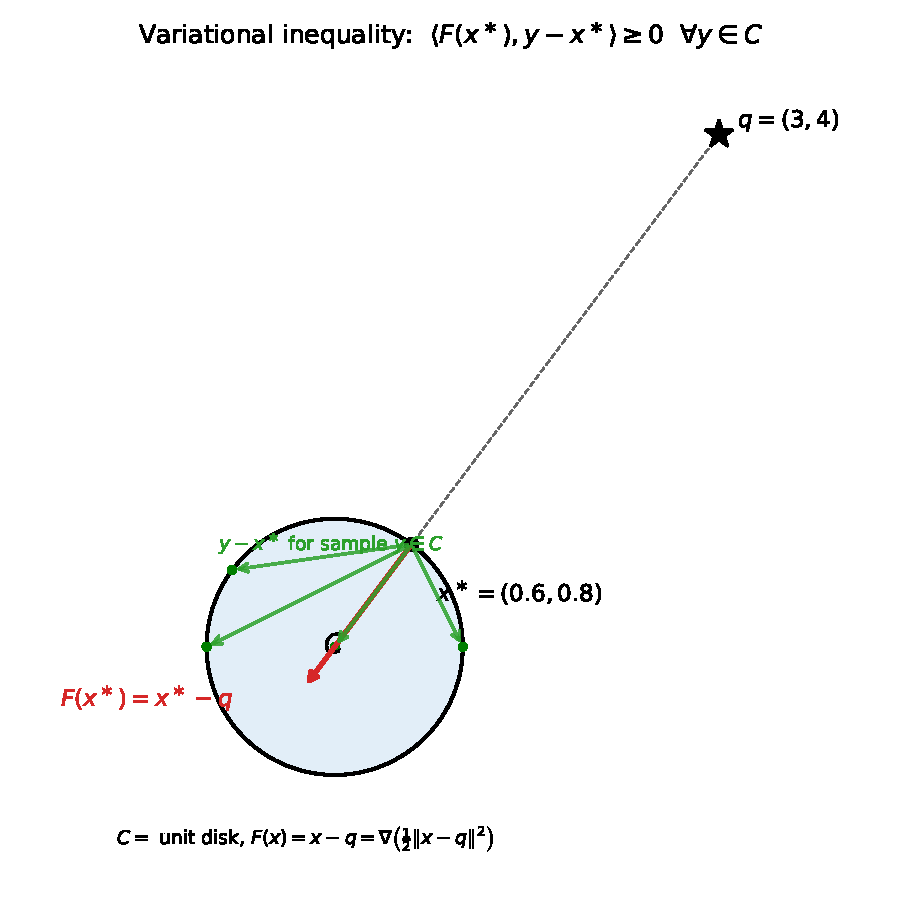
\includegraphics[width=0.62\textwidth]{fig_vi_diagram}
  \end{center}
  \footnotesize $C$ is the unit disk, $F(x)=x-q=\nabla\bigl(\tfrac12\norm{x-q}^2\bigr)$.
  The solution $x^*$ of the VI is exactly $P_C(q)$ --- the same
  point $(0.6,0.8)$ from the running example, now arising as the
  minimizer of $\tfrac12\norm{x-q}^2$ over $C$. At $x^*$, the vector
  $F(x^*)$ makes a non-obtuse angle with $y-x^*$ for \emph{every}
  feasible $y\in C$ (green arrows), which is precisely the VI
  condition $\inner{F(x^*)}{y-x^*}\ge0$.

\end{frame}

%==============================================================
\section{Chapter Summary}
%==============================================================

\begin{frame}{Chapter 7 Summary}

  \begin{block}{What we learned}
    \begin{itemize}
      \item The \textbf{optimal relaxation parameter} $\widehat\lambda_{p,n}$
            (Eq.\ 7.9) minimizes $\norm{x_{n+1}-p}$ exactly, but
            requires the unknown fixed point $p$ --- it is a
            theoretical benchmark, generalizing Combettes'
            $\lambda_n^*$ (Eq.\ 7.1) for $T=P_DP_S$.
      \item Substituting $T(x_n)$, $T^2(x_n)$ for $p$ gives the
            \textbf{computable approximation} (Eq.\ 7.12), provably
            convergent under mild safeguards (Theorems 7.3--7.6).
      \item The \textbf{fixed-point / VI equivalence}
            ($F=\Id-T$, Lemmas 7.3--7.4) lets any relaxation
            strategy invented for variational inequality projection
            methods be imported into KM iterations --- illustrated
            by Algorithms 5, 6, 7 (Tseng-type, line-search, and
            golden-ratio variants).
      \item The \textbf{residual algorithm} (Algorithm 8) chooses
            $\lambda_n=\rho_n\mu_n$ via a backtracking line search
            on the fixed-point residual, combined with a
            Barzilai--Borwein-style spectral coefficient $\rho_n$,
            converging under a (fairly strong) compactness
            assumption.
      \item On the \textbf{running example} (unit-disk projection,
            $x_0=(3,4)$), the ideal and practical optimal-parameter
            formulas coincide exactly and reach $x^*=(0.6,0.8)$ in a
            single step --- versus a slow geometric approach for
            fixed $\lambda=0.5$ --- illustrating, in the simplest
            possible setting, why adaptive relaxation matters.
      \item \textbf{Open problems remain}: convergence of the
            unsafeguarded approximate sequence (7.12), and joint
            optimal choice of inertial \emph{and} relaxation
            parameters together.
    \end{itemize}
  \end{block}

\end{frame}

\end{document}
